
\documentclass[a4paper,english,12pt]{article}
\usepackage{%
	amsfonts,%
	amsmath,%	
	amssymb,%
	amsthm,%
	algorithm,%
	babel,%
	bbm,%
	etex,%
	%biblatex,%
	caption,%
	centernot,%
	color,%
	dsfont,%
	enumerate,%
	epsfig,%
	epstopdf,%
	geometry,%
	graphicx,%
	hyperref,%
	latexsym,%
	mathtools,%
	multicol,%
	pgf,%
	pgfplots,%
	pgfplotstable,%
	pgfpages,%
	proof,%
	psfrag,%
	subfigure,%	
	tikz,%
	ulem,%
	url%
}	
\usepackage[noend]{algpseudocode}
\usepackage[mathscr]{eucal}
\usepgflibrary{shapes}
\usetikzlibrary{%
  	arrows,%
	backgrounds,%
	chains,%
	decorations.pathmorphing,% /pgf/decoration/random steps | erste Graphik
	decorations.text,%
	matrix,%
  	positioning,% wg. " of "
  	fit,%
	patterns,%
  	petri,%
	plotmarks,%
  	scopes,%
	shadows,%
  	shapes.misc,% wg. rounded rectangle
  	shapes.arrows,%
	shapes.callouts,%
  	shapes%
}

\theoremstyle{plain}
\newtheorem{thm}{Theorem}[section]
\newtheorem{lem}[thm]{Lemma}
\newtheorem{prop}[thm]{Proposition}
\newtheorem{cor}[thm]{Corollary}

\theoremstyle{definition}
\newtheorem{defn}[thm]{Definition}
\newtheorem{conj}[thm]{Conjecture}
\newtheorem{exmp}[thm]{Example}
\newtheorem{assum}[thm]{Assumptions}
\newtheorem{axiom}[thm]{Axiom}

\theoremstyle{remark}
\newtheorem{rem}{Remark}
\newtheorem{note}{Note}
\newtheorem{fact}{Fact}

\newcommand{\norm}[1]{\left\lVert#1\right\rVert}
\newcommand{\indep}{\!\perp\!\!\!\perp}
\DeclarePairedDelimiter\abs{\lvert}{\rvert}%
\newcommand\numberthis{\addtocounter{equation}{1}\tag{\theequation}}
\newcommand{\tr}{\operatorname{tr}}
\newcommand{\R}{\mathbb{R}}
\newcommand{\N}{\mathbb{N}}
\newcommand{\E}{\mathbb{E}}
\newcommand{\Z}{\mathbb{Z}}
\newcommand{\B}{\mathscr{B}}
\newcommand{\C}{\mathcal{C}}
\newcommand{\T}{\mathscr{T}}
\newcommand{\F}{\mathcal{F}}
\newcommand{\G}{\mathcal{G}}
%\newcommand{\ba}{\begin{align*}}
%\newcommand{\ea}{\end{align*}}
\DeclareMathOperator*{\argmax}{arg\,max}
\renewcommand{\qedsymbol}{$\blacksquare$}
\makeatletter
\def\BState{\State\hskip-\ALG@thistlm}
\makeatother

\makeatletter
\def\th@plain{%
  \thm@notefont{}% same as heading font
  \itshape % body font
}
\def\th@definition{%
  \thm@notefont{}% same as heading font
  \normalfont % body font
}
\makeatother
\date{}

%opening
\title{Lecture-11: Detection of Deterministic Signals in Gaussian Noise}
\author{}

\begin{document}
\maketitle
\noindent The basic problem that we are dealing is the following hypothesis testing problem : 
\begin{equation}
\label{ht}
     \begin{aligned}
     & H_0 : Y_k=N_k+S_{0k} ,\ \ \ \ k=1,2,3,...n  \\
      \mbox{versus} & \\
       & H_1 : Y_k=N_k+S_{1k} ,\ \ \ \ k=1,2,3,...n
     \end{aligned}
\end{equation}


In the previous lectures, we have seen the cases where noise samples $N_k$ were i.i.d. If the noise samples $N_k$ in \eqref{ht} are not independent of each other, then the likelihood ratio 
\begin{equation}
L(\underline{y})=\frac{E \lbrace p_N(\underline{y}-\underline{S}_1)\rbrace}{E \lbrace p_N(\underline{y}-\underline{S}_0)\rbrace}  \ \ \  \ y\in \R^ n
\end{equation}
do not exhibit any particular structure, even for the case of deterministic signals.\\
An important exception for this lack of structure is the situation in which the signals are deterministic$(\underline{S}_j=\underline{s}_j)$ and the noise vector $\underline{N}$ has multivariate Gaussian distribution. In this case, the optimum detectors have simple, easily implemented structures and  performance of the optimum systems can be analyzed thoroughly. Thus it is of interest to consider this case in detail.\\
Let  $\underline{S}_j \ \mbox{for} \ j=\lbrace 0,1 \rbrace$, take known values say, $\underline{s}_0,\underline{s}_1 \in \R ^n$ and that noise vector $\underline{N}$ is a Gaussian random vector with mean vector $\underline{0}$ and covariance matrix $\sum_N$. That is,
\begin{equation}
\underline{N} \sim \mathcal{N} \Big(\underline{0}, \sum\nolimits_N \Big)
\end{equation}
The assumption of zero mean noise does not reduce the generality of the results since we can always subtract a non zero noise mean from $\underline{y}$ to produce a new observation with zero mean noise.\\
A Gaussian random vector in $\R^n$ with mean vector  $\underline{\mu} \triangleq \mathbb{E}\lbrace\underline{X} \rbrace \in \R^n$ and $n \times n $ covariance matrix $\sum \triangleq \mathbb{E} \lbrace (\underline{X}-\underline{\mu})(\underline{X}-\underline{\mu})^T \rbrace$ has probability density function 
\begin{equation}
p_{\underline{X}}(\underline{x})=\dfrac{1}{(2\pi)^{n/2} \vert \sum \vert ^{1/2}  } \exp \lbrace -\frac{1}{2} (\underline{x}-\underline{\mu})^T \sum\nolimits^{-1} (\underline{x} - \underline{\mu}) \rbrace \ \ \ \ \underline{x} \in \R ^n 
\end{equation}
where $\vert \sum \vert $ denotes the determinant of $\sum$ and $\sum ^{-1}$ denotes the inverse of $\sum$.\\
We will assume that $\sum _N$ is positive definite. That is, $\underline{x}^T\sum_{N} \underline{x} > 0 \ \forall \ \underline{x} \in \R ^n-\{\underline{0}\}$. Positive definiteness of $\sum_{N}$ implies that $\vert \sum_{N} \vert > 0$ and $\sum ^{-1} $ exists.\\

The received vector $\underline{Y}$ has a Gaussian distribution with $\underline{s}_j$ as the mean and $\sum _N$ as the covariance matrix, that is, $\underline{Y} \sim \mathcal{N}(\underline{s}_j,\sum_N), \ j \in \lbrace 0,1 \rbrace$. The likelihood ratio for the received $\underline{y}$ can be written as 
\begin{align*}
\centering
L(\underline{y})=\dfrac{p_1(\underline{y})}{p_0 (\underline{y})} &=
\dfrac{\dfrac{1}{(2\pi)^{n/2} \vert \sum_N \vert ^{1/2}  } \exp \lbrace -\frac{1}{2} (\underline{y}-\underline{s}_1)^T \sum\nolimits^{-1}_N (\underline{y} - \underline{s}_1) \rbrace}{\dfrac{1}{(2\pi)^{n/2} \vert \sum_N \vert ^{1/2}  } \exp \lbrace -\frac{1}{2} (\underline{y}-\underline{s}_0)^T \sum\nolimits^{-1}_N (\underline{y} - \underline{s}_0) \rbrace}  \\
\vspace{0.2 cm}
&= \exp\Big \lbrace \underline{s}_1^T \sum\nolimits_N^{-1} \underline{y} - \underline{s}_0^T \sum\nolimits_N^{-1} \underline{y} -\frac{1}{2}\underline{s}_1^T \sum\nolimits_N^{-1} \underline{s}_1 + \frac{1}{2}\underline{s}_0^T \sum\nolimits_N^{-1} \underline{s}_0 \Big \rbrace\\ 
\vspace{0.25 cm}
\mbox{Since} \ \sum\nolimits _N  \ &\mbox{and hence} \  \sum\nolimits_N^{-1} \mbox{are symmetric matrices} , \ 
\underline{s}_j^T \sum\nolimits_N^{-1}\underline{y} = \underline{y}^T\sum\nolimits _N^{-1} \underline{s}_j  .
\end{align*}

Hence the expression for $L(\underline{y})$ is
\begin{equation}
\label{LR}
L(\underline{y})= \exp \Big\{ (\underline{s}_1-\underline{s}_0)^T \sum\nolimits_N^{-1} \Big( \underline{y} - \frac{\underline{s}_0+\underline{s}_1}{2} \Big) \Big\} \ \ \ \ \underline{y} \in \R ^n
\end{equation}

We observe that the problem under consideration is the vector version of the simple location testing problem studied earlier, where the locations $\mu _0$ and $\mu _1$ are replaced with location vectors $\underline{s}_0 \ \mbox{and} \ \underline{s}_1$ and the noise variance $\sigma ^2$ is replaced with noise covariance matrix $\sum_N$.\\
Taking logarithm on both sides of \eqref{LR} we get,
$$
\log L(\underline{y}) = (\underline{s}_1-\underline{s}_0)^T\sum\nolimits_N^{-1} \Big(\underline{y} - \dfrac{\underline{s}_0 + \underline{s}_1}{2} \Big)
$$  
Here, $\frac{1}{2}(\underline{s}_1-\underline{s}_0)^T \sum_N^{-1}(\underline{s}_0+\underline{s}_1)$ does not depend on $\underline{y}$. Hence it can be incorporated into the decision threshold. The optimum test becomes

\begin{align}
\tilde{\delta}_0 (\underline{y}) =  
\begin{cases}
1 &>  \\
\gamma  \ \ \ \  (\underline{s}_1-\underline{s}_0)^T \sum\nolimits_N^{-1} \underline{y} &= \tau' \\
0 &<
\end{cases}
\label{dr}
\end{align}
where $\tau'=\log\tau + \frac{1}{2}(\underline{s}_1-\underline{s}_0)^T \sum_N^{-1} (\underline{s}_0+\underline{s}_1)$.\\ We can write
\begin{equation}
(\underline{s}_1-\underline{s}_0)^T \sum\nolimits_N^{-1} \underline{y}=\tilde{\underline{s}}^T\underline{y}=\sum_{k=1}^n \tilde{s}_ky_k
\end{equation}
where $\tilde{\underline{s}}=\sum_N^{-1}(\underline{s}_1-\underline{s}_0)$ is called \textit{derived signal} or \textit{impulse response} of matched filter.\\
Now, the detector structure is identical to the optimum detector for coherent signals in i.i.d Gaussian noise with the actual signal $\underline{s}$  replaced by the ``pseudo signal" $\tilde{\underline{s}}$. Hence the implementation of detector is no more difficult for dependent noise than for independent noise.

\section{Performance of the Detector:}
Observe that the quantity
$
T(\underline{Y}) \triangleq (\underline{s}_1-\underline{s}_0)^T \sum\nolimits_N^{-1}\underline{Y}
$ 
is a linear transformation of the Gaussian random vector $\underline{Y}$. A basic property of the multivariate Gaussian distribution is that, linear transformation of Gaussian vectors are also Gaussian. In this case, since the transformation is to $\R$, $T(\underline{Y})$ is a Gaussian random variable. The distribution of $T(\underline{Y})$ under $H_0$ and $H_1$ can be completely characterized by finding its means and variances under the two hypothesis.\\
Under $H_j$, the mean of $T(\underline{Y})$ is given by
\begin{align}
\mathbb{E} \{ T(\underline{Y} | H_j) \} &= \mathbb{E}\{\tilde{\underline{s}}^T\underline{Y} | H_j \} = \tilde{\underline{s}}^T \mathbb{E}\{ \underline{Y} | H_j \} \nonumber  \\
  &= \tilde{\underline{s}}^T \mathbb{E} \{\underline{s}_j + \underline{N} |H_j \} \nonumber \\
 &=\tilde{\underline{s}}^T \mathbb{E} \{\underline{N}|H_j \} + \tilde{\underline{s}}^T\underline{s}_j \nonumber \\
  &= \tilde{\underline{s}}^T\underline{s}_j \triangleq \tilde{\mu}_j, \ \ j \in \{ 0,1 \} 
 \label{pd}
\end{align}   

 Similarly, the variance of $T(\underline{Y})$ under $H_j$ is 
\begin{align}
Var\{T(\underline{Y} )| H_j\} & = \E \{(\tilde{\underline{s}}^T \underline{Y} - \tilde{\underline{s}}^T \underline{s}_j)^2 | H_j \} \nonumber \\
& =\E\{(\tilde{\underline{s}}^T \underline{N})^2 \} \nonumber \\
& =\E\{\tilde{\underline{s}}^T \underline{N}\underline{N}^T \tilde{\underline{s}} \} \nonumber \\
& = \tilde{\underline{s}}^T \E \{\underline{N}\underline{N}^T \} \tilde{\underline{s}} \nonumber \\
& =\tilde{\underline{s}}^T \sum\nolimits_N \tilde{\underline{s}} \nonumber \\ 
 & = (\underline{s}_1-\underline{s}_0)^T \sum\nolimits _N^{-1} (\underline{s}_1-\underline{s}_0)  \triangleq d^2
\end{align}

Note that the variance of $T(\underline{Y})$ is independent of the hypothesis. Also, the positive definiteness of $\sum _N$ implies that $\sum _N^{-1}$ is also positive definite and thus $d^2 >0$ unless $\underline{s}_1 = \underline{s}_0$. Thus, $T(\underline{Y}) \sim \mathcal{N}(\tilde{\mu}_j,d^2)$ under $H_j$ for $j=\{0,1\}$. Since $T(\underline{Y})$ is continuous, there is no need for randomization. Hence $\gamma$ in \eqref{dr} is irrelevent. 

\begin{align}
P_j(\Gamma_1) &= \dfrac{1}{\sqrt{2\pi d^2}} \int_{\tau'}^{\infty} e^{-(x-\tilde{\mu}_j)/2d^2} dx \nonumber \\
&=1-\Phi \Big( \dfrac{\tau' - \tilde{\mu}_j}{d} \Big)
\label{pg1}
\end{align}
\noindent where $d$ is the positive square root of $d^2$ and $\Phi(\cdot)$ is the cdf of standard Gaussian distribution. $P_j(\Gamma_1)$ can be written in terms of the original threshold $\tau$ as

\begin{equation}
P_j(\Gamma_1) = 
\begin{cases}
1-\Phi \Big(\dfrac{\log \tau}{d} + \dfrac{d}{2} \Big) &\mbox{for}~j=0\\
1-\Phi \Big(\dfrac{\log \tau}{d} - \dfrac{d}{2} \Big) &\mbox{for}~j=1.
\end{cases}
\end{equation}  
It can be observed that the Bayesian performance in the problem under consideration here is identical to the location testing problem with $n=1$. Similarly, the performance for the Minimax and Neyman-Pearson problems under consideration here is identical to the location testing problem studied earlier.

\begin{exmp}
For Neyman-Pearson testing with false alarm probability of $\alpha$, 
$P_{FA}(\tilde{\delta})=\alpha = P_0(\Gamma_1)$. From \eqref{pg1} we see that
\begin{equation}
\alpha = 1- \Phi \Big( \dfrac{\tau'-\tilde{\mu}_0}{d} \Big)
\end{equation} 
The corresponding detection probability is 
\begin{align*}
P_D (\tilde{\delta}_{NP}) =P_1(\Gamma_1) &= 1- \Phi \Big( \dfrac{\tau'-\tilde{\mu}_1}{d} \Big) \\
&= 1-\Phi \Big( \dfrac{d\Phi^{-1}(1-\alpha) + \tilde{\mu}_0 - \tilde{\mu}_1}{d} \Big) \\
&=1-\Phi\Big( \Phi^{-1}(1-\alpha) + \dfrac{\tilde{\mu}_0 - \tilde{\mu}_1}{d} \Big) \\
\end{align*}

\begin{align*}
\dfrac{\tilde{\mu}_0 - \tilde{\mu}_1}{d} &= \dfrac{\tilde{\underline{s}}^T\underline{s}_0 - \tilde{\underline{s}}^T\underline{s}_1}{d} \\
&=\dfrac{\Big[ \sum\nolimits_N^{-1} (\underline{s}_1-\underline{s}_0) \Big]^T(\underline{s}_0-\underline{s}_1)}{d} \\
&= \dfrac{(\underline{s}_1 - \underline{s}_0)^T \sum\nolimits_N^{-1} (\underline{s}_0 - \underline{s}_1)}{d} = -d
\end{align*}
Therefore, the expression for detection probability is
\begin{equation}
P_D(\tilde{\delta}_{NP})=1-\Phi (\Phi ^{-1} (1-\alpha) - d)
\end{equation}

\end{exmp}
\begin{note}
$P_D(\tilde{\delta}_{NP})$ is a monotonically increasing function in $d$ as shown in Fig. \ref{pNP}.
\begin{figure}[hbtp]
\centering
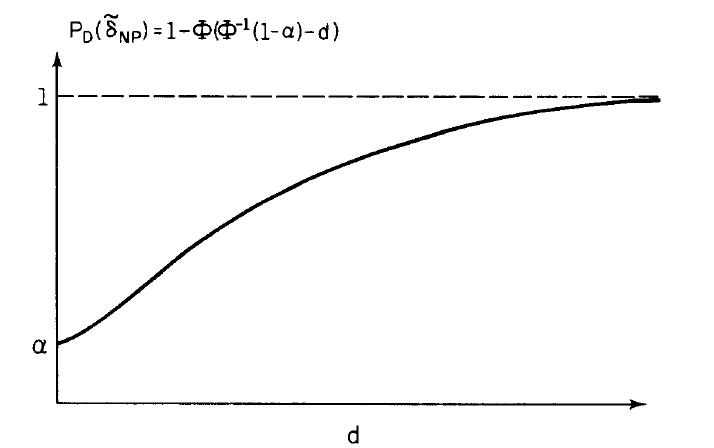
\includegraphics[scale=0.75]{Figures/pd.jpeg}
\caption{Power function for Neyman pearson test with Gaussian error \\ \textit{(Source: H. Vincent Poor, An Introduction to Signal Detection and Estimation(Second
Edition), Figure II.D.3)}}
\label{pNP}
\end{figure}
Higher the value of $d$, better is the detection probability.
\end{note}


\begin{note}\textbf{\underline{Interpretation of $d^2$}}\\
$d^2$ can be interpreted as a measure of signal to noise ratio. Consider the case when $\underline{s}_0=\underline{0}$ and $\underline{s}_1=\underline{s}$.\\

\noindent \textit{Case 1:} When noise is i.i.d $\mathcal{N}(0,\sigma ^2)$ which corresponds to the multivariate Gaussian case with $\sum_N=\sigma^2I$, where $I$ denotes $n\times n$ identity matrix.\\
In this case
\begin{align}
\sum\nolimits_N^{-1} = \sigma^{-2}I \nonumber \\
d^2 &=(\underline{s}_1-\underline{s}_0)^T \sum\nolimits_N^{-1} (\underline{s}_1-\underline{s}_0) \nonumber \\
&=\dfrac{\underline{s}^TI\underline{s}}{\sigma^2} \nonumber \\
&=\dfrac{1}{\sigma^2}\sum_{k=1}^{n}s_k^2=\dfrac{n\bar{s}^2}{\sigma^2}
\end{align}
where $\bar{s}^2 \triangleq \dfrac{1}{n}\sum\limits_{k=1}^n s_k^2$ is the average signal power, $\sigma^2 = \dfrac{1}{n} \sum\limits_{k=1}^n \E \{N_k^2 \}$ is the average noise power, so that $d^2$ is the product of average signal to noise power and the number of samples.\\

\noindent  \textit{Case 2:} A similar interpretation can be given to $d^2$ in non i.i.d case. Matched filter output for pure signal($\underline{s}$) at time $n$ is
$$\tilde{\underline{s}}^T \underline{s}=\underline{s}^T \sum\nolimits_N^{-1}\underline{s}=d^2$$
Therefore, signal power at the output of matched filter at  time $n$ is $d^4$. Matched filter output power for input equal to pure noise($\underline{N}$) at time $n$ is $$\E\{(\tilde{\underline{s}}^T \ \underline{N})^2\}= \underline{s}^T\sum\nolimits_N^{-1}\underline{s}=d^2$$
Hence
$$
\dfrac{\mbox{signal power at the output of matched filter}}{\mbox{noise power at the output of matched filter}} = \dfrac{d^4}{d^2} =d^2
$$

\end{note}

\vspace{1 cm}
\begin{note}
Matched filter output at time $n$ is nothing but multiplication by $\tilde{s}^T$. We can write the quantity $\sum\limits_{k=1}^n \tilde{s}_ky_k$ as the input at time $n$ of an LTI filter with impulse response   
\begin{equation}
\tilde{h}_k= \begin{cases}
\tilde{s}_{n-k} & 0 \leq k \leq n-1\\
0 &\mbox{otherwise}.
\end{cases}
\label{ir}
\end{equation}
The filter $\tilde{h}$ of \eqref{ir} has maximum output SNR at time $n$ among all linear filters with impulse response of length $n$.
 \end{note}
\vspace{1 cm}

\begin{note}
The quantity $d^2 $ also has another interpretation for the i.i.d case with general signals $\underline{s}_0, \underline{s}_1$ and $\underline{N} \sim \mathcal{N}(\underline{0}, \sigma^2 I)$. In this case, we can write
$$
d^2=\dfrac{1}{\sigma^2} \norm{\underline{s}_1-\underline{s}_0}^2_2
$$

\noindent where $\norm{\underline{s}_1-\underline{s}_0}$ denotes Euclidean distance between the signal vectors. Thus, the farther apart the signal vectors are, the better performance can be achieved.
\end{note}

\section{Reduction to the i.i.d noise case}
The observation vector $\underline{Y}$ can be transformed to give an equivalent observation with i.i.d noise. In particular, because $\sum_N$ is positive definite, it can be written as
\begin{equation}
\sum\nolimits_N = CC^T
\label{cholskey}
\end{equation}
\noindent where $C$ is an $n \times n $ invertible lower triangular matrix. Eq. 
\ref{cholskey} is called \textit{Cholesky decomposition} of $\sum_N$.
\begin{align*}
&\sum\nolimits_N = CC^T\\
&(\sum\nolimits_N)^{-1} = (CC^T)^{-1}=(C^T)^{-1}C^{-1} \\
\mbox{Let} \ &D \triangleq C^{-1}, \ \mbox{then} \\
&\sum\nolimits_N^{-1} = D^TD, \ \ \mbox{$D$ is also lower triangular} \\
\mbox{Let} \  &\underline{\bar{Y}} \triangleq D\underline{Y}=D\underline{s}_j + D\underline{N}\\
&\bar{D} \triangleq D\underline{s}_j \ \ \mbox{is the transformed signal and} \\
&\underline{\bar{N}} \triangleq D\underline{N} \ \ \mbox{is the transformed noise} 
\end{align*}
Clearly,
\begin{align*}
 \E \{D\underline{N}\} &= \underline{0} \\
Var\{D \underline{N}\} &= \E \{ D\underline{N} \ \underline{N}^T D^T \} \\
&=D\sum\nolimits_N D^T = C^{-1} \sum\nolimits_N(C^{-1})^T \\
&=\sum\nolimits_N \sum\nolimits_N^{-1}=I 
\end{align*}

\noindent Hence, $\underline{\bar{N}} \sim \mathcal{N}(\underline{0},I)$. So, we now have an i.i.d noise situation and the optimum detection statistic is 
\begin{align*}
T(\underline{Y}) &=(\underline{s}_1 - \underline{s}_0)^T\sum\nolimits_N^{-1}\underline{Y} \\
&=(\underline{s}_1 - \underline{s}_0)^T D^T D \underline{Y} \\
&=(\underline{\bar{s}}_1 - \underline{\bar{s}}_0)^T \underline{\bar{Y}}
\end{align*}

\noindent Note that the lower triangularity of $C$ implies that $C^{-1}$ is also lower triangular.\\
Cholesky decomposition is preferred because, $\underline{\bar{Y}}=C^{-1}\underline{Y}$ can be implemented as the output at times $(0,1,....,n-1)$ of a causal (time varying) filter. Since the noise in the output of this filter is white (i.i.d), this filter is sometimes known as \textit{whitening filter}. So, the optimim decoder can be represented as follows.  

\begin{figure}[hbtp]
\centering
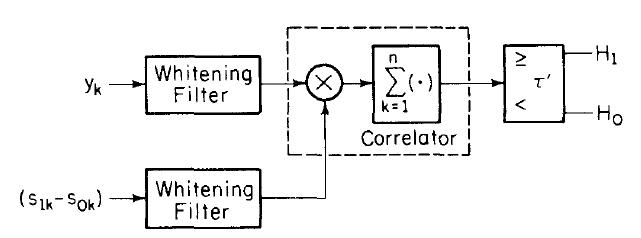
\includegraphics[scale=0.75]{Figures/VP_III_B_8.jpeg}
\caption{Optimum detector for coherent signals in dependent Gaussian noise \\ \textit{(Source: H. Vincent Poor, An Introduction to Signal Detection and Estimation(Second
Edition), Figure III.B.8)}}
\label{vp_III_B_8}
\end{figure}

\noindent The performance of coherent detection in dependent noise depends on how far apart the signals are when transformed to a coordinate system in which the noise components are i.i.d.

\section{Optimal Signal Design}
The performance of optimum coherent detection in Gaussian noise is improved by increasing the quantity $d^2 \triangleq (\underline{s}_1 - \underline{s}_0)^T \sum_N^{-1} (\underline{s}_1 - \underline{s}_0)$. We consider designing signal $\underline{s}_1=\underline{s}$ such that these signals maximize $d^2$ given $noise \sim \mathcal{N}(\underline{0},\sum_N)$.\\
Consider $\alpha-$ level N-P detection 
$$ P_D(\tilde{\delta}_{NP}) = 1-\Phi(\Phi^{-1}(1-\alpha) -d)$$
We have the following problem,
\begin{equation}
\max_{\underline{s}} d^2 = \underline{s}^T \sum\nolimits_N^{-1} \underline{s} \ \ \  \mbox{s.t} \ \norm{s}^2_2 \leq E
\end{equation}
\noindent where $E$ is the energy/power constraint.\\

\noindent If $\lambda_1, \lambda_2, ....,\lambda_n$ are eigen values of $\sum_N$, since $\sum_N$ is symmetric, we can find orthonormal eigen vectors $\underline{v}_1, \underline{v}_2,......,\underline{v}_n$ corresponding to eigen values $\lambda_1,\lambda_2,......,\lambda_n$ respectively. $\sum_N$ can be expanded as
\begin{align*}
\sum\nolimits_N &=\sum_{i=1}^{n}\lambda_i \underline{v}_i \underline{v}_i^T \\
\underline{x}^T \sum\nolimits_N^{-1} \underline{x} &= \underline{x}^T (\sum_{i=1}^{n} \lambda_i^{-1} \underline{v}_i\underline{v}_i^T)\underline{x} \\
&=\sum_{i=1}^n \lambda_i^{-1} \underline{x}^T \underline{v}_i\underline{v}_i^T \underline{x} \\
&\leq \sum_{i=1}^n (\lambda_{min}^{-1})\underline{x}^T\underline{v}_i\underline{v}_i^T \underline{x}=\lambda_{min}^{-1} \norm{\underline{x}}^2_2 \nonumber\\
&\leq \lambda_{min}^{-1}E
\end{align*}
\noindent The solution is by setting 
$$\underline{s}=c \underline{v}_k \ \ \mbox{s.t} \ \lambda_k = \lambda_{min} \ \ \mbox{with} \ \ \norm{\underline{s}}^2_2 = c^2=E $$
Therefore,
\begin{align*}
d_{opt}^2 &=\underline{s}^T \sum\nolimits_N^{-1}\underline{s}  \\
&=\sqrt{E} \underline{v}_k^T \sum\nolimits_N^{-1} \underline{v}_k \sqrt{E}\\
&= \dfrac{E}{\lambda_{min}}
\end{align*}
\noindent The optimum detection probability for $\alpha-$ level N-P test with power constraint $E$ is 
\begin{equation}
1P_{D,opt}=1-\Phi\left(\Phi^{-1}(1-\alpha) - \sqrt{\dfrac{E}{\lambda_{min}}}\right)
\end{equation}

\end{document}